\documentclass[document.tex]{subfiles}
\begin{document}

\chapter{Literature Review}

\section{Introduction}
\noindent Relevant feature identification has become an essential task to apply data mining algorithms effectively in real-world scenarios. Therefore, many feature selection methods have been proposed to obtain the relevant feature or feature subsets in the literature to achieve their objectives of classification and clustering.
The amount of high-dimensional data that exists and is publically available on the internet has greatly increased in the past few years. Therefore, machine learning methods have difficulty in dealing with the large number of input features, which is posing an interesting challenge for researchers. In order to use machine learning methods effectively,pre-processing of the data is essential. Feature selection is one of the most frequent and important techniques in data pre-processing, and has become an indispensable component of the machine learning process. It is also known as variable selection, attribute selection, or variable subset selection in machine learning and statistics. It is the process of detecting relevant features and removing irrelevant, redundant, or noisy data. This process speeds up data mining algorithms, improves predictive accuracy, and increases
comprehensibility. Irrelevant features are those that provide no useful information, and
redundant features provide no more information than the currently selected features.
\section{Feature Mining}

\section{Related Works}

\section{Feature Relevancy and Redundancy}

\section{General Approach for Feature Selection}

\section{Feature Mining for Hyperspectral Image}

\section{Classification Techniques}
\noindent Digital image classification techniques group pixels to represent land cover features. Land cover could be forest, urban, agricultural and other types of features. There are two main image classification techniques.
\begin{itemize}
	\item Unsupervised Classification
	\item Supervised Classification
\end{itemize}
\subsection{Unsupervised Classification}
\noindent Pixels are grouped based on the reflectance properties of pixels. These groupings are
called "clusters". The user identifies the number of clusters to generate and which bands
to use. With this information, the image classification software generates clusters. There
are different image clustering algorithms such as K-means and ISODATA.
Unsupervised classification is a method which examines a large number of unknown pixels and divides into a number of classed based on natural groupings present in the image values. unlike supervised classification, unsupervised classification does not require
analyst-specified training data. The basic premise is that values within a given cover
type should be close together in the measurement space (i.e. have similar gray levels),
whereas data in different classes should be comparatively well separated (i.e. have very
different gray levels) (PCI, 1997; Lillesand and Kiefer, 1994; Eastman, 1995 )
The classes that result from unsupervised classification are spectral classed which based on natural groupings of the image values, the identity of the spectral class will not be initially known, must compare classified data to some from of reference data (such as larger
scale imagery, maps, or site visits) to determine the identity and informational values
of the spectral classes. Thus, in the supervised approach, to define useful information
categories and then examine their spectral separability; in the unsupervised approach the
computer determines spectrally separable class, and then define their information value.
(PCI, 1997; Lillesand and Kiefer, 1994)

\begin{figure}[H]
	\begin{center}
		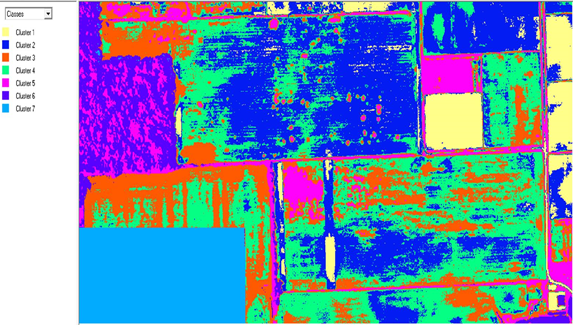
\includegraphics[height=6.0cm]{imgs/Unsupervised.png}
	\end{center}
	\caption{Unsupervised Classification}
	\label{fig: Unsupervised Classification}
\end{figure}
Unsupervised classification is becoming increasingly popular in agencies involved in
long term GIS database maintenance. The reason is that there are now systems that use
clustering procedures that are extremely fast and require little in the nature of operational parameters. Thus it is becoming possible to train GIS analysis with only a general
familiarity with remote sensing to undertake classifications that meet typical map accuracy standards. With suitable ground truth accuracy assessment procedures, this tool can provide a remarkably rapid means of producing quality land cover data on a continuing basis.
\subsection{Supervised Classification}
\noindent The user selects representative samples for each land cover class in the digital image.
These sample land cover classes are called "training sites". The image classification
software uses the training sites to identify the land cover classes in the entire image.
The classification of land cover is based on the spectral signature defined in the training set. The digital image classification software determines each class on what it resembles
\begin{figure}[H]
	\begin{center}
		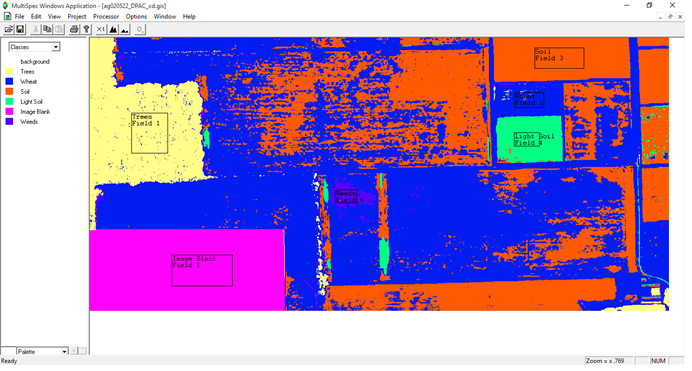
\includegraphics[height=6.0cm]{imgs/Supervised.png}
	\end{center}
	\caption{Supervised Classificationn}
	\label{fig: Supervised Classification}
\end{figure}
most in the training set. The common supervised classification algorithms are maximum
likelihood and minimum-distance classification.
\end{document}